\documentclass{aa}  
%\documentclass[longauth]{aa}   % for the long lists of affiliations
%\documentclass[letter]{aa}     % for the letters

\usepackage{amsmath}
\usepackage{float}
\usepackage{graphicx}
\usepackage{txfonts}
\usepackage{lipsum}
\usepackage{stfloats}
\usepackage{siunitx}
\usepackage{adjustbox}
\usepackage{booktabs}
\usepackage{subcaption}         % necessary for continued figures, example in section 3
                                % and appendix
\usepackage{lscape}             % to rotate a single page table, example in appendix.
                                % For landscape tables, see the longtable examples.
\usepackage{placeins}           % useful with \FloatBarrier, to keep 
                                % onecolumn floats from drifting to the next section
\usepackage{hyperref}
\hypersetup{
    colorlinks=true,
    linkcolor=blue,
    citecolor=blue,
    filecolor=magenta,      
    urlcolor=blue,
}
% \usepackage[breaklinks=true,colorlinks=true,
%             linkcolor=black,citecolor=blue,urlcolor=black]{hyperref}

\usepackage{multicol, float}

\DeclareSIUnit\year{yr}


\begin{document}

% \title{Astronomy \& Astrophysics \LaTeX\ template}
% \title{Understanding Giant Planet Properties Across Stellar Environments}
%\title{Investigating the Significance and Impacts of Theoretical Uncertainties on Giant Planet Bulk Properties}
\title{The impact of theoretical models on our understanding of giant exoplanets}
% \subtitle{Subtitle}


\author{
    Anshak Mallik\inst{1}
% \fnmsep\thanks{Shows the usage of elements in the author field}
    \and Simon M\"uller\inst{1}
    \and Ravit Helled\inst{1}
}

\institute{
    Department of Astrophysics, University of Z\"urich, Winterthurerstrasse 190, 8057 Z\"urich, Switzerland
}

\date{Received April XX, 2026}
 
\abstract
% context heading (optional)
% {} leave it empty if necessary  
{The characterisation of giant exoplanet compositions relies on thermal evolution models. However, the sensitivity of inferred bulk metallicities to different modelling frameworks is poorly quantified, often leading to significant differences in the planetary characterisation.}
% aims heading (mandatory)
{We aim to evaluate how differences in theoretical models, specifically the treatment of the atmosphere, equations of state, and statistical inference, impact the planetary characterisation and the inferred population-wide metallicity trends.} 
% methods heading (mandatory)
{We inferred the bulk metallicities of a sample of 80 gas giants from 0.1 to 3 Jupiter masses using two different publicly available thermal evolution models. We compared these results to previous studies that used different thermal models and inference methods. We analysed the variations in their underlying assumptions, including hydrogen-helium equation of states and  atmospheric models.}
% results heading (mandatory)
{We find systematic shifts in the absolute bulk metallicity estimates across models, primary driven by differences in atmospheric models and the treatment of the atmosphere-interior boundary. However, despite these offsets, the different models reconstruct a consistent negative correlation between planetary mass and bulk metallicity.}
% conclusions heading (optional), leave it empty if necessary
{Theoretical uncertainties introduce significant systematic shifts in the characterisation of individual planets. However, population-wide insights, especially the mass-metallicity relation, are robust to model variations. We recommend that these theoretical uncertainties should be considered when interpreting ongoing and future exoplanetary data.}

\keywords{
    Planets and satellites: composition,  --
    Planets and satellites: gaseous planets --
    Planets and satellites: interiors
}

\maketitle


\section{Introduction}\label{sec:introduction}
The bulk composition of giant planets is regarded as a fingerprint of their formation and evolutionary pathways \citep[e.g.,][]{Helled2014,Johansen2017,Ginzburg2020}. According to the core accretion model \citep{Mizuno1980,pollack_formation_1996}, the amount and distribution of the heavy elements in a gas giant are determined by the efficiency of solid accretion and timing of gas envelope acquisition \citep[e.g.,][]{ 2017ApJ...840L...4H,lozovsky_jupiters_2017,valletta_deposition_2019}. Therefore, the inference of bulk metallicites and studying them on a population level is an important contributor to better understanding the origin of giant planets.

In the last decades, space-based transit missions and ground-based radial velocity follow-ups provided a large and diverse population of exoplanets with accurately measured masses $M_p$ and radii $R_p$. This facilities the inference of the planetary bulk composition and internal structure \citep[e.g.,][]{fortney_planetary_2007,seager_mass-radius_2007, spiegel_structure_2014,jontof-hutter_compositional_2019,muller_towards_2023}, which yielded in the now well-established mass-metallicity relation of giant planets \citep{thorngren_mass-metallicity_2016,teske_metal-rich_2019,muller_bulk_2025,peerani_how_2025}.

The inferred planetary bulk metallicity $Z_p$, however, depends on the assumed physics, especially the used Equations of State (EoS),the atmospheric boundary conditions and opacities and the numerical details of the inference \citep{2008A&A...482..315B, vazan_effect_2013,2019Atmos..10..664P,howard_accounting_2023,howard_giant_2025}. Consequently, the field has reached a point where the reported metallicity of a planet may often be more a reflection of the chosen computational tool. Independent studies now often report divergent bulk metallicites for the same planet, leading to difficulties in their interpretation \citep{thorngren_mass-metallicity_2016,muller_bulk_2025,chachan_revising_2025}. The diversity in underlying assumptions would make a direct cross-comparison inconsistent, highlighting exactly the aforementioned issue. Given all this, it is important to understand the origin and implications of these differences. 

In this work, we performed a controlled comparison of four independent interior modelling tools. Rather than only focusing on the specific value of $Z_p$ of individual planets, we quantified the systematic shifts caused by the use of different models and their assumptions. Next, we tested whether the mass-metallicity relation remains consistent across different model assumptions, numerical tools and statistical frameworks.

Our paper is organised as follows. In Section 2, we describe the planetary sample and the four interior modelling tools used in this comparison. Section 3 presents our results, focusing on the systematic shifts in the bulk metallicity and robustness of the mass-metallicity relation across different model assumptions. We discuss tthe the physical implications of these discrepancies in Section 4. Finally, our conclusions and outlook for future population studies are summarised in Section 5.


\section{Methods}\label{sec:methods}
The bulk metallicity\footnote{The bulk metallicity refers to the mass fraction of heavy elements in the planet.} of giant planets is commonly inferred by combining the measured mass, radius, and age with thermal evolution models that predict the cooling. This achieved by using the model to find which heavy-element mass would yield a predicted radius that is consistent with the observations (at the right age). \citep[e.g.,][]{fortney_planetary_2007,thorngren_mass-metallicity_2016}. Since the measurements have associated uncertainties, a Monte Carlo approach is usually employed, resulting in an estimate of the posterior distribution of the total-heavy element mass or bulk metallicity. A simple way to do this is to construct prior distributions informed by observations and then repeatedly using a root-finding method to match the sampled radius, therefore obtaining an estimate of the bulk metallicity posterior \citep[e.g.,][]{thorngren_mass-metallicity_2016,muller_towards_2023}. A more computationally involved approach is to run a full Markov Chain Monte Carlo (MCMC) retrieval for the bulk metallicity, which again yields estimates of the posterior distribution \citep[e.g.,][]{acuna_characterisation_2021,sing_warm_2024, ashtari_gems_2026}.

In this work, we used two different public thermal evolution models to estimate the bulk metallicity of a large sample of giant exoplanets. We briefly describe these models and the planetary sample in the upcoming subsections \ref{sec:thermal_evolution_models} and \ref{sec:planet_catalogue}. We also used two previously published results as an additional comparison, and we describe the details of the models that were used in Subsection \ref{sec:additional_models}.


\subsection{Thermal evolution models}\label{sec:thermal_evolution_models}
The first thermal evolution model used in this work was a modified version \citep{helled_giant_2025} of the stellar evolution code Modules for Experiments in Stellar Astrophysics (\texttt{MESA}; \citet{paxton_modules_2011,paxton_modules_2013,paxton_modules_2018,paxton_modules_2019,jermyn_modules_2023}). The relevant modifications are an enhancement of the standard \texttt{MESA} equation of state, which now include the \citet{chabrier_new_2021} hydrogen-helium equation of state, and a 50-50 water-rock mixture for the heavy elements using the QEOS \citep{more_new_1988,vazan_effect_2013}.

Similar to the \texttt{planetsynth} models from \citet{muller_synthetic_2021}, we used a $T-\tau$ atmosphere accounting for the irradiation flux, the radiative opacities from \citet{freedman_gaseous_2014}, and assumed a proto-solar heavy-element mass fraction in the envelope. We can calculated a large grid of models varying the planetary mass $M_p$, irradiation flux $I_p$, and bulk metallicity $Z_p$. We then constructed an interpolator on that grid with \texttt{scipy.interpolate.RegularGridInterpolator} to serve as the forward model for estimating the bulk metallicities. 
% This estimate was done in a full MCMC framework using \texttt{emcee} \citep{foreman-mackey_emcee_2013}

The second thermal evolution model used here was \texttt{GASTLI} \citep{acuna_gastli_2024}. The code calculates a series of static one-dimensional structure models, and then separately connects them to the thermal evolution via the integration of the luminosity equation. 

The inference analysis was conducted identically as mentioned above with the core mass fraction (CMF) being sampled instead of $Z_p$. Using values of from \cite{muller_bulk_2025} as an initial estimate was used to draw $Z_p$ samples from a uniform distribution.

% The \texttt{GASTLI} code \citep{acuna_gastli_2024} was used for the thermal evolution of planets. This code numerically solves the 1D equations that describe the interior structure and thermal evolution equations, coupled to equations of state (EoS). The interior consists of two distinct regions: a core surrounded by a gaseous envelope. The atmosphere is defined as the region above the boundary of the interior at $P_{\text{surf}} = 1000\: \si{\bar}$. 

% Previous studies, such as \cite{howard_giant_2025} investigated  how the choice of the EoS affect the thermal evolution and the inference of planetary properties. 
% \texttt{GASTLI} uses the following EoS: SESAME \citep{lyon_sesame_1992} for silicate in the core, CD21 \citep{chabrier_new_2021} for H/He in the envelope, M19 \citep{mazevet_ab_2019} \& AQUA \citep{haldemann_aqua_2020} for pure water in the envelope and atmosphere.
% In this work, we focus on the H/He species and note that \texttt{GASTLI} uses the CD21 EoS \citep{chabrier_new_2021} for hydrogen and helium in the envelope. The atmospheric model is \texttt{petitCODE} \citep{molliere_model_2015}.

The results of thermal evolution sequences used to generate a grid with dimensions of core mass fraction $\text{CMF}$, mass $M_p\: [M_J]$, equilibrium temperature $T_{\text{eq}}\: [\si{\kelvin}]$
% internal temperature $T_{\text{int}}\: [\si{\kelvin}]$. 
and age $\tau_p\: [\si{\giga\year}]$.
The remaining results of the thermal evolution sequences were overlayed on this grid and we implemented linear interpolation (\texttt{scipy.interpolate.RegularGridInterpolator}). The envelope metallicity was set constant to solar value $Z_{\text{env}} = Z_{\odot} = 0.014$ \citep{lodders_abundances_2009, ekstrom_grids_2012}. A grid was also created with the thermal evolution sequences similar to what was previously described. 

For the inference of bulk metallicity $Z_p$, the standard Markov Chain Monte Carlo (MCMC) approach was employed, similarly to \cite{muller_bulk_2025}. Mass $M_p$, core mass fraction $\text{CMF}$ and age $\tau_p$ were the planetary parameters drawn by sampling prior distributions from observations.
% \textbf{Mass, radius and age were the planetary parameters drawn by sampling prior distributions from observations.}
The mass was sampled from normal distribution based on observations, $\text{CMF}$ sampled from a uniform distribution bounded between $0.01$ and $0.9$ and age was sampled from a uniform distribution between the minimum and maximum observed stellar age. The lowest possible age was limited to $1\: \si{\giga\year}$, while the upper age limit was set to $13.6\: \si{\giga\year}$, the age of the Milky Way. Thus, for each planet there is a unique parameter sample space. On each of these, an ensemble of 32 walkers were evolved for 10000 draws in order to obtain posterior distribution for $\text{CMF}$. Using this, we obtained distributions for bulk metallicity using $Z_p = \text{CMF} + Z_{\text{env}}(1-\text{CMF})$.


The second model we considered is \texttt{planetsynth}  \citep{muller_synthetic_2021}. This model also solves planetary equations for interior structures and thermal evolution coupled with a set of EoS. The EoS for H/He was modified to also use CD21, instead of CMS19 \citep{chabrier_new_2019} as in the initial version of the tool. Envelope metallicity was set at $Z_{\text{env}} = 0.012$ and with a grey atmosphere using opacities from \citep{freedman_gaseous_2014}.

The inference analysis was conducted identically as mentioned above for \texttt{GASTLI} with $Z_p$ being sampled instead of $\text{CMF}$. Using values of from \cite{muller_bulk_2025} as an initial estimate was used to draw $Z_p$ samples from a uniform distribution.


\subsection{Planet catalogue}\label{sec:planet_catalogue}
The planetary sample used here is the same as in \citet{muller_bulk_2025}, which is based on the PlanetS catalogue \citep{parc_super-earths_2024} with a few additional recently detected planets around M-dwarf stars \citep{hartman_toi_2024,2024AJ....168..235K}. We only considered warm Jupiters with equilibrium temperatures of $T_{\text{eq}} \le 1000\: \si{\kelvin}$ and masses between 0.1 and 3 M$_{\rm{J}}$. These selection criteria lead to a total sample size of 80 exoplanets.


\subsection{Additional models for comparison}\label{sec:additional_models}
\subsubsection{Reference 1: P25}
The first study we refer to is P25 \citep{peerani_how_2025}, which used \texttt{CEPAM} \citep{guillot_cepam_1995} as the thermal evolution tool. This also assumes a simple core and envelope structure for giant planets. Specifically for this study, the choice for the H/He EoS was CMS19 + HG23 \citep{chabrier_new_2019, howard_accounting_2023} which is similar to the CD21 EoS. Additionally, the atmospheric model is Parmentier's non-grey model \citep{parmentier_non-grey_2015} with an envelope metallicity of $Z_{\text{env}} = 0$. This combination also makes it similar to the solar value.

For the inference of $Z_p$, a root-finding method was employed. 5000 draws of the mass, radius and age were used per planet to find the root of a function that is constrained by the observed radius.


\subsubsection{Reference 2: T19}
Another reference study is T19 \citep{teske_metal-rich_2019}. Both thermal evolution and inference methods follow the same exact procedure as in T16 \citep{thorngren_mass-metallicity_2016}. For this, a private thermal evolution tool is used which is not publicly available. For the evolution, the SvCH \citep{saumon_equation_1995} EoS for H/He is applied. 
% \textbf{The Fortney atmospheric model is used for the boundary condition.}

% \textbf{NOTE: i am unsure what the assigned envelope metallicity is and what kind of atmospheric model the Fortney model is.}
As mentioned, the inference method is the exact same as in T16. This is similar to our methods used for results from \texttt{GASTLI} and \texttt{planetsynth}.
\medskip
% \break

To ensure a fair comparison, we focus on a core sample of 6 planets that are common in all four planet catalogues. Note that the complete catalogues for P25 and T19 contain 43 and 33 exoplanets respectively. All above-mentioned information is also summarised in Tab.~\ref{tab:EoS_and_atm_model}.

\begin{table*}[!t]
    \centering
    \begin{tabular}{lllll}
    \hline
    \hline
    Reference & TE Tool           & H/He EoS      & $Z_{\text{env}}$ & Atmospheric Model        \\
    \hline
    - & \texttt{GASTLI}      & CD21          & 0.014            & \texttt{petitCODE} \\
    - & \texttt{planetsynth} & CD21          & 0.012            & Freedman? (grey)                   \\
    P25   & \texttt{CEPAM}    & CMS19 + HG23* & 0*               & Parmentier*                \\
    T19   & private               & ScVH (T16)    & ?                & Fortney?                  \\
    \hline
    \end{tabular}
    \caption{TODO}
\label{tab:EoS_and_atm_model}
\end{table*}


%%%%%%%%%%%%%%%%%%%%%%%%%%%%%%%%%%%%%%%%%%%%%%%%%%%%%%%%%%%%%%
% \clearpage
\section{Results}

\subsection{Bulk Metallicity Posterior Distributions}
The inference of bulk metallicities of giant planets is sensitive to the assumptions of the thermal evolution tools used. Fig.~\ref{fig:3.1_bulk_metallicity_comparison_TE_tools} illustrates the posterior distributions for six representative gas giants that are available in our catalogue, as well as those that have been investigated in the aforementioned studies.

\begin{figure*}[!t]
  \centering
  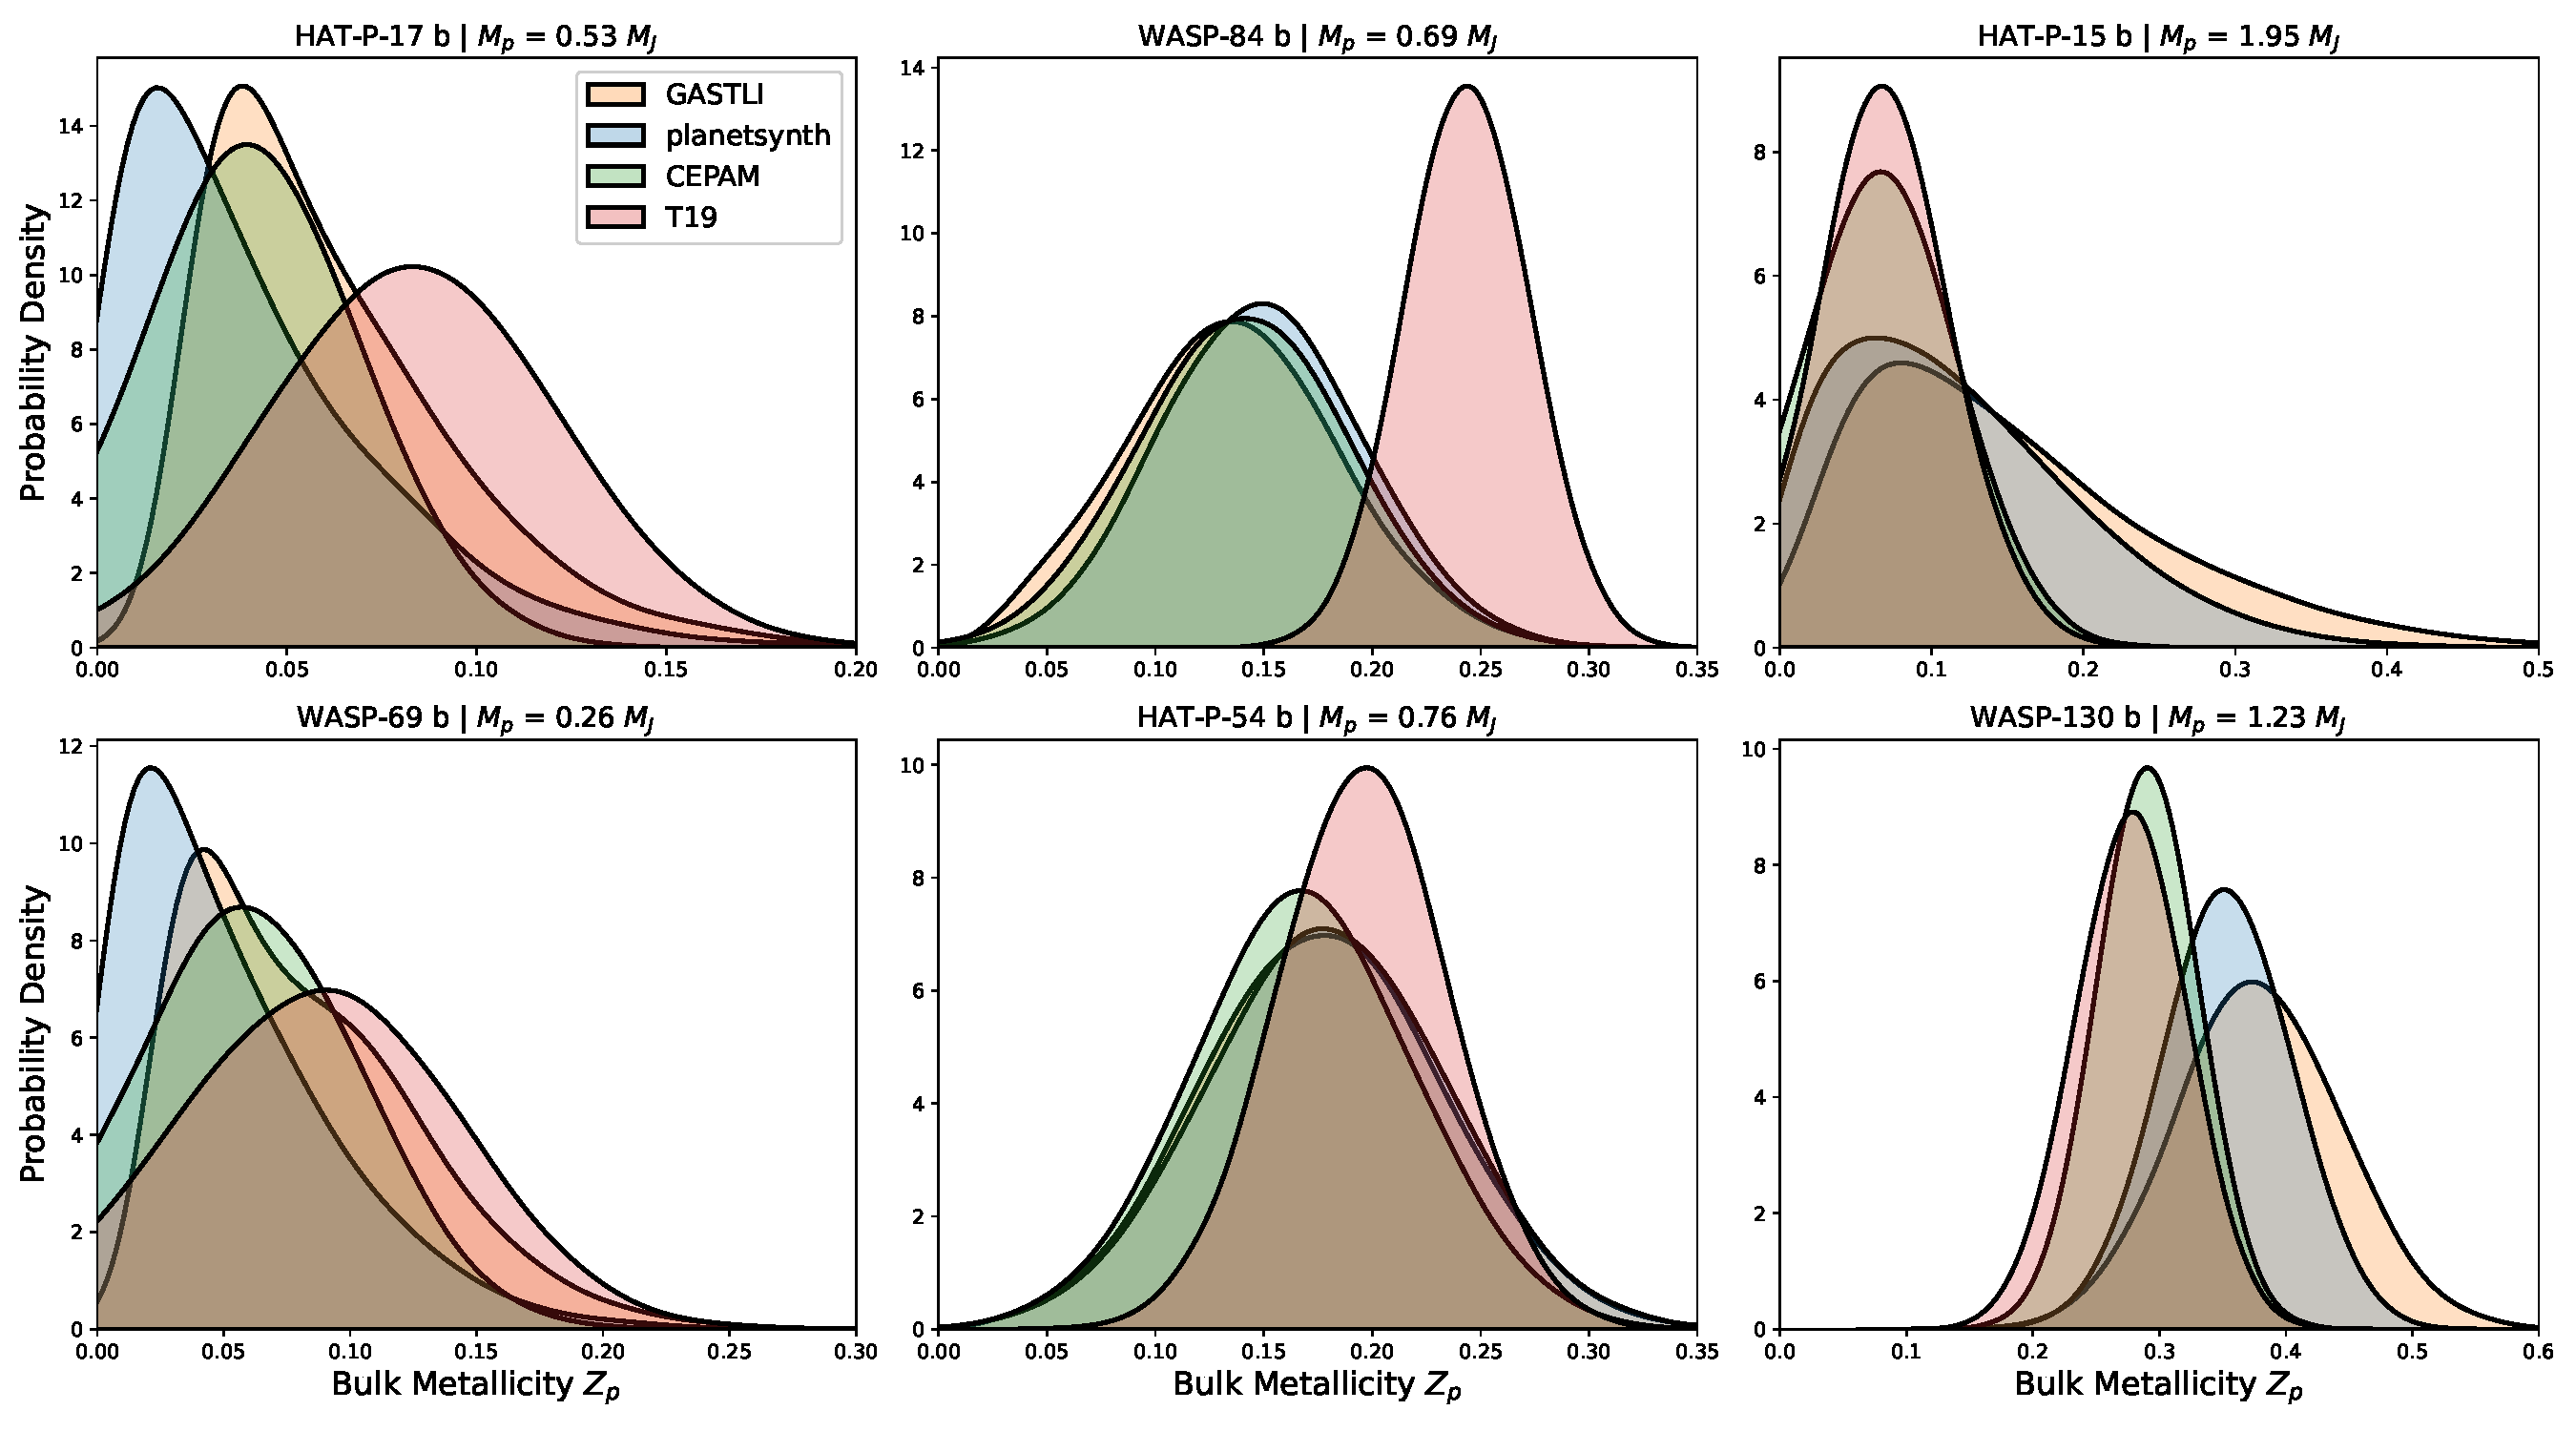
\includegraphics[width=\hsize]{fig/3.1_bulk_metallicity_comparison_4_datasets_cepam_teske_new_fill.pdf}
  \caption{Posterior distributions of inferred bulk metallicities $Z_p$ of six planets from the catalogue. The distributions representing results from \texttt{GASTLI} (orange) and \texttt{planetsynth} (blue) are obtained following a standard MCMC procedure, initialised with 10000 draws per planet. The raw results were used, leading to skewed distributions. Results from T19 (green) followed the same analysis method. However, since raw data was not available, the results from the study were assumed to follow a normal distribution. Results from P25 (red) followed a root-finding method and only used 5000 initial draws per planet. They were also assumed to follow a normal distribution, as the raw data was not available. The lower legend denotes estimates for the heavy-element mass $M_Z$ obtained from the global mode of the posterior distributions $Z_p$.}
  \label{fig:3.1_bulk_metallicity_comparison_TE_tools} 
\end{figure*}

A primary observation in Fig.~\ref{fig:3.1_bulk_metallicity_comparison_TE_tools} is the difference in the morphologies of the posterior distributions. Results of \texttt{GASTLI} and \texttt{planetsynth} exhibit skewed, non-Gaussian distributions. This skewness is a byproduct of the MCMC procedure of 10000 initial draws, which captures the physical non-linearities of the interior structures. On the other hand, those from P25 and T19 appear as symmetric normal distributions despite following similar sampling procedures (10000 and 5000 initial draws, respectively). This is because the raw data from the studies was unavailable, and thus symmetric errors were assumed for these distributions.

For the individual planets, the primary observation is the systematic shifts of the peak of bulk metallicity $Z_p$ between tools. While the EoS for rocks and water, which represent metals, were different, the EoS for H/He were very similar. Consistent H/He EoS across thermal evolution models lead to a more consistent $Z_p$ prediction. So, while the EoS for H/He might have slight differences, they are not the primary cause for the shifts in peaks. This can be attributed to the atmospheric models used in each thermal evolution tool. These are indeed very different from each, and the transition from a radiative atmosphere to convective interior significantly impacts how the planet would have evolved. This also includes how the envelope is treated, and if it is assumed to be homogeneous and convective, what value is assigned to $Z_{\text{env}}$. These differences across thermal evolution models are highlighted in Tab.~\ref{tab:EoS_and_atm_model}.


\subsection{Bulk Metallicity Trends}
The individual distributions of $Z_p$ in Fig.~\ref{fig:3.1_bulk_metallicity_comparison_TE_tools} highlight tool-specific uncertainties. However, with increasing mass in the mass range $M_p \in [0.01,\ 3] M_J$ reveals a consistent negative trend in bulk metallicity $Z_p$. The magnitude and slope are sensitive to the thermal evolution tool employed. These trends are visualised in Fig.~\ref{fig:3.2_trend_comparison}.

% \clearpage
\begin{figure*}
  \centering
  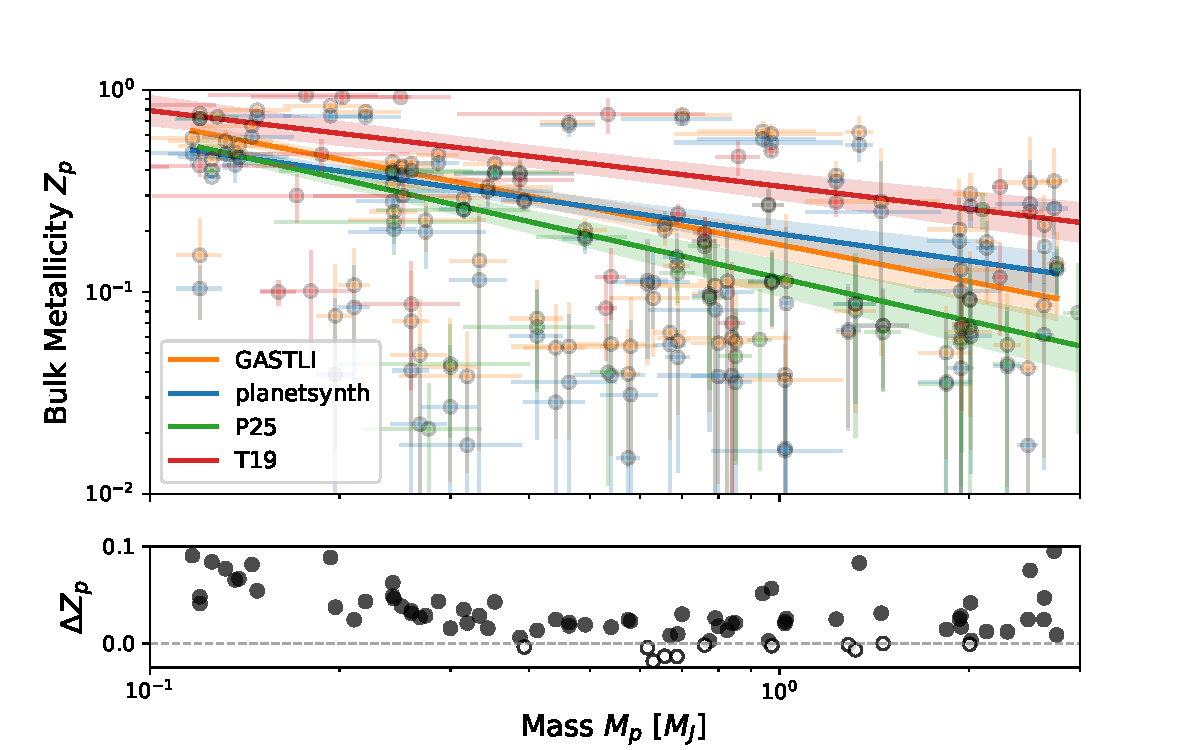
\includegraphics[width=\hsize]{fig/3.2_trend_comparison_new.pdf}
  \caption{Inferred bulk metallicity $Z_p$ as a function of planetary mass for $M_p \in [0.01, 3]\, M_J$. \textit{Top panel}: Scatter points and error bars show inferred values for bulk metallicity. The solid lines are their respective fits constructed using orthogonal distance regression. Shaded areas around these lines are the $1\sigma$ uncertainties of this fit. \textit{Bottom panel}: Residuals of the inferred bulk metallicity values between the two thermal evolution tools. These are calculated by subtracting the \texttt{planetsynth} values from the \texttt{GASTLI} values. Blank points represent planets which had \texttt{planetsynth} predict a higher $Z_p$ than \texttt{GASTLI}.}
  \label{fig:3.2_trend_comparison}
\end{figure*}

The top panel of Fig.~\ref{fig:3.2_trend_comparison} shows the orthogonal distance regression fit for the 4 models. Each fit follows a slightly different slope, but all of them are negative. The bottom panel showcases the difference in \texttt{GASTLI}'s and \texttt{planetsynth}'s results for $Z_p$. \texttt{GASTLI} tends to predict higher bulk metallicities, except for exactly eleven planets shown in red. 
  

%%%%%%%%%%%%%%%%%%%%%%%%%%%%%%%%%%%%%%%%%%%%%%%%%%%%%%%%%%%%%%
% \clearpage
\section{Discussion}

% \clearpage
\subsection{Talking Points about Differences}
Divergences in the inferred bulk metallicities across the four evolution tools highlight how significant the role of model noise plays in the characterisation of exoplanets. 

\subsubsection{Structure \& EoS}
A fundamental factor to consider is the treatment of the planetary structure. All four mentioned evolutions assume a standard core+envelope architecture with a homogeneous and convective envelope. However, the definition of metals and the materials used to represent them vary:

\begin{itemize}
    \item{\textbf{Material Modelling:} the choice of modelling heavy elements as pure rock (silicates), water or a mixture creates offsets in the bulk density calculations. Since the EoS for these materials differs across the tools, the inferred metallicity required to match observed radii measurements will fluctuate, despite identical H/He EoS.}
    \item{\textbf{H/He:}} Since giant planets are primarily composed of H and He, the choice of their EoS significantly impacts the inference of their bulk properties. While the results from \texttt{GASTLI} and \texttt{planetsynth} are consistent with each other (CD21) and very similar to P25 (CMS19+HG23), T19 still utilises ScVH. This can lead to a variety in compressibility gradients. Thus, even slight variations in the density at large pressures are followed by significant shifts in $Z_p$ to match the observed radius.
\end{itemize}
% \newpage

\subsubsection{Inference Methods}
The statistical approach used to infer $Z_p$ also dictates the shifts in the results.
\begin{itemize}
    \item{\textbf{MCMC Sampling:} The inference done for \texttt{GASTLI}, \texttt{planetsynth} and T19 utilised MCMC procedures with 10000 steps. This allowed for a full exploration of the parameter space, capturing the skewed nature of the posterior distributions. This approach is limited by multiple observational constraints (mass, age, radius).}
    \item{\textbf{Root-Finding:} In contrast, P25 employed a root-finding method. Thus the model is limited to only a single observational constraint, the radius. This could also explain why the posterior distributions tend to be narrower.}
\end{itemize}


\subsubsection{Systematic Shifts vs. Robust Trends}
Despite the existence of systematic shifts in the individual values of $Z_p$, the most vital takeaway is should be the difference between absolute shifts and relative trends.
\begin{itemize}
    \item{\textbf{Model Shifts:} An example of absolute and systematic shifts is portrayed in the bottom panel of Fig.~\ref{fig:3.2_trend_comparison}. It shows that \texttt{GASTLI} trends to predicts higher metallicites than \texttt{planetsynth}, particularly at lower masses. This could be explained by the differences in the atmospheric boundary conditions.}
    \item{\textbf{Agreement on Trends:} One should notice that in spite of these shifts, all four tools reconstruct a similar negative trend for the mass-metallicity relation. This indicates that while tools may not agree with each other on the exact amount of heavy elements present in a planet, they do agree that with increasing mass giant planets are less likely to be heavily enriched in metals. This means they are in agreement of efficiency of metal enrichment during the planet formation proceess across mass scales.}
\end{itemize}

\subsection{Consistency in Scaling Planetary Radii}
A source of a systematic error in exoplanetary characterisation might arise from the inconsistent use of Jupiter's reference radius. Observations typically report planetary radii scaled to the equatorial radius of Jupiter ($R_{J, \text{eq}} = 11.20\, R_{\oplus}$). Meanwhile, some thermal evolution and interior characterisation tools might scale according to the volumetric mean radius of Jupiter ($R_{J, \text{eq}} = 10.97\, R_{\oplus}$). 

It is essential for the reference radius to be consistent across observations and analysis frameworks to ensure self-consistent retrieval. The framework within \texttt{GASTLI} already uses $R_{J,\text{eq}}$ for radius conversions. To highlight the impact this choice of radius has, we look at the impact of working with inconsistent radii conversions. For this, we manually scale the radius values by the factor $k_J = R_{J,\text{mean}} / R_{J,\text{eq}} \approx 0.98$, leading to a smaller radius than observed. This inconsistency leads to a systematic bias in the inferred bulk properties. To quantify this effect, we compared retrievals on \texttt{GASLTI} for the planet K2-114 b, as seen in Fig.~\ref{fig:3.3_corner_plot_comparison_overlay}.

\begin{itemize}
  \item{\textbf{Consistent}: Observations and analysis radii are scaled into Juipter radii with the equatorial radius $R_{J,\text{eq}}$.}
  \item{\textbf{Inconsistent}: Observations follow $R_{J,\text{eq}}$, whereas the analysis manually rescales radii to use the volumetric mean radius $R_{J,\text{mean}}$.}
\end{itemize}

\begin{figure}[h]
  \centering
  % 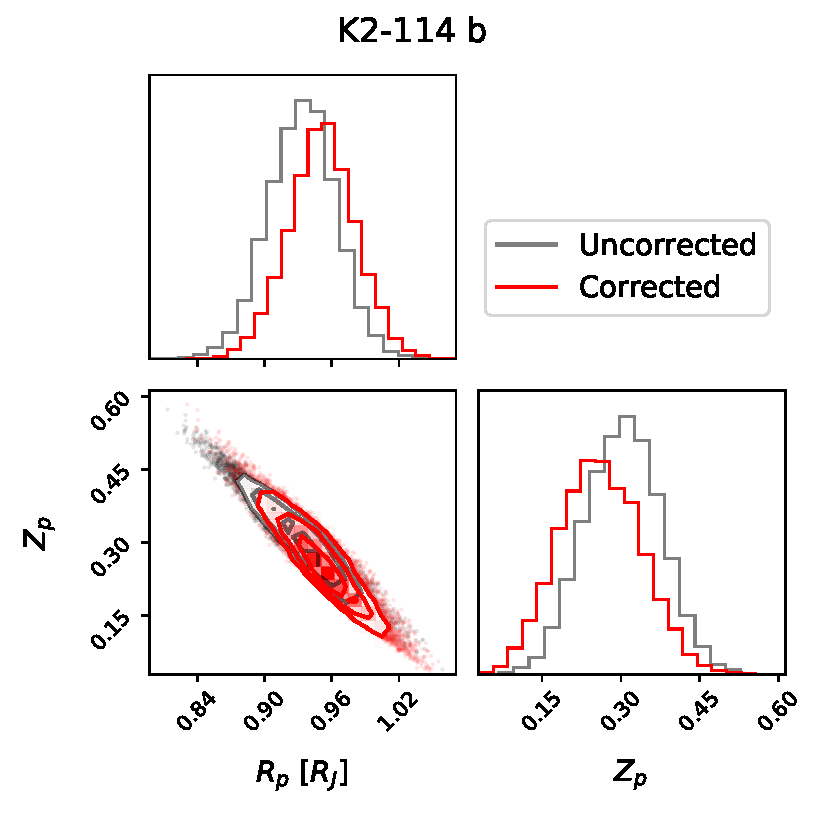
\includegraphics[width=\hsize]{fig/3.3_corner_plot_comparison_overlay.pdf}
  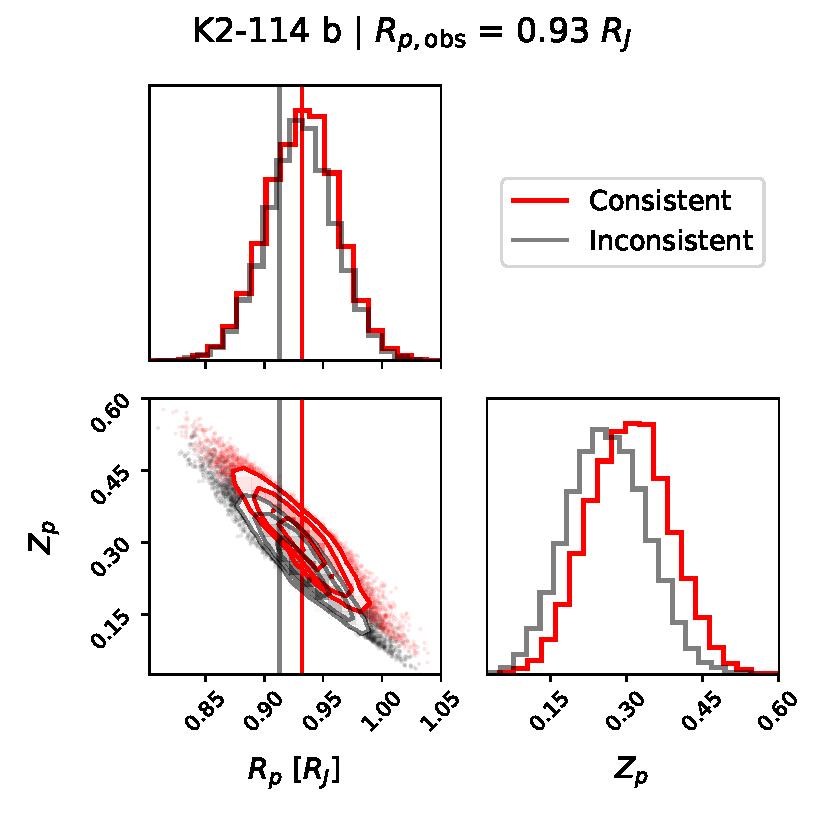
\includegraphics[width=\hsize]{fig/3.3_corner_plot_comparison_overlay_new.pdf}
  \caption{Posterior distributions for the radius $R_p$ and bulk metallicity $Z_p$ of K2-114 b with observed radius $R_{p,\text{obs}} = 0.93^{+0.03}_{-0.03}\, R_J$, following the equatorial radius. Vertical lines represent in the first plot represent the ``true'' radius value $R_p$ used for the analysis. The red contours represent the consistent retrieval which also utilises the equatorial radius: $R_p = R_{p,\text{obs}}$. The gray contours represent the inconsistent retrieval which scales according to the volumetric mean radius: $R_p <  R_{p,\text{obs}}$. The shift towards a lower $Z_p$ in the inconsistent case demonstrates the impact of the radius value on inferred composition.}
  \label{fig:3.3_corner_plot_comparison_overlay}
\end{figure}

As seen in Fig.~\ref{fig:3.3_corner_plot_comparison_overlay}, both cases assume different values for the ``true'' radius based on the reference Jupiter radius used. In the consistent case, the true radius already matches the observed value ($R_{p,\text{obs}} = 0.93^{+0.03}_{-0.03}\, R_J$) and yields an inferred bulk metallicity of $Z_p = 0.31^{+0.08}_{-0.08}$. However, in the inconsistent case the true radius is smaller than the observed value ($R_{p,\text{obs}} = 0.91^{+0.03}_{-0.03}\, R_J$). The MCMC sampler is forced to predict a higher radius in order to match the observation, yielding a lower inferred bulk metallicity of $Z_p = 0.26^{+0.08}_{-0.08}$. Thus, the price for overestimating radii to match observation is paid by having to underestimate the inferred bulk metallicity.
 %concrete numbers: 0.02 R_J increase in radius leads to 0.05 decrease in Zp -> mention? if yes, how do we justify this?

% \textbf{TODO: mention that P25 used inconsistent scaling? if yes, talk about how this inconsistent scaling affects root-finding functions the same way it does for MCMC sampling methods}





%%%%%%%%%%%%%%%%%%%%%%%%%%%%%%%%%%%%%%%%%%%%%%%%%%%%%%%%%%%%%%
\section{Summary \& Conclusions}
We compared the inferred bulk metallicities of gas giants using \texttt{GASTLI} and \texttt{planetsynth} with a standard MCMC sampling procedure. The results were also compared to P25 and T19. Our main conclusions can be  summarised as follows:
\begin{itemize}
    \item{There are systematic shifts in the bulk metallicity estimates and they stem from different model assumptions, such as the used atmospheric models and EoS.}
    \item{We tried working with consistent H/He EoS, while the EoS of rock and water varied significantly across all four tools. As H and He are the most abundant elements in the envelope of gas giants, it is more important to ensure that at least their EoS is consistent. Only in T19 was an older EoS used for H/He.}
    \item{The choice of inference between MCMC sampling and root-finding methods also affects the results. The method of root-finding  is limited to one observational constraint only. MCMC sampling, on the other hand, uses multiple observational constraints allowing  for a more extended exploration of the parameter space.}
    \item{Despite the shifts in individual estimates of the planetary bulk metallicity, the inferred trend of the decreasing mass-metallicity relation is robust.}
    %This confirms that population-level insights are robust to variations across models.}
    \item{Systematic biases can arise from inconsistent planetary radius scaling. The discrepancy between using Jupiter's equatorial versus volumetric mean radius as a reference can introduce a shift in the input radius. As demonstrated with K2-114 b, this inconsistency forces the model to compensate for the radius difference by underestimating the bulk metallicity by shifting the inferred composition $Z_p$ as much as 0.05.}
\end{itemize}
%Currently, the community tends to overlook the significance of the theoretical uncertainties. As a community, we could either move towards a more standardised approach , or simply put more emphasis on these uncertainties and include them in discussions in more detail. It might also be interesting to replicate this study for different types of interior structures, that are not limited to the simple core+envelope model. 
% Additionally, facilities such as JWST might increase observational precision. As this would help refine internal boundary conditions and 
Ultimately, as we enter an era of high-precision spectroscopy with facilities like JWST and Ariel, the bottleneck for understanding giant planets may no longer be the quality of our observations, but the limitations of our theoretical frameworks. Our study demonstrates that while individual bulk metallicity estimates remain sensitive to the choice of atmospheric boundary conditions and equations of state, the overarching trends of planetary formation remain visible through the modeling noise. By acknowledging and quantifying these systematic shifts, we can better calibrate our expectations, ensuring that our search for the origins of giant planets is built upon a transparent and robust theoretical foundation.



%%%%%%%%%%%%%%%%%%%%%%%%%%%%%%%%%%%%%%%%%%%%%%%%%%%%%%%%%%%%%%
% \begin{acknowledgements}
%       Part of this work was supported by \emph{ESO}, project
%       number Ts~17/2--1. \citep{acuna_characterisation_2021}
% \end{acknowledgements}


%%%%%%%%%%%%%%%%%%%%%%%%%%%%%%%%%%%%%%%%%%%%%%%%%%%%%%%%%%%%%%
\bibliographystyle{aa}
\bibliography{references,referencesmanual}
% \printbibliography


%%%%%%%%%%%%%%%%%%%%%%%%%%%%%%%%%%%%%%%%%%%%%%%%%%%%%%%%%%%%%%
% WARNING
% Please note that we have included the references below in
% order to compile the document, but we ask you to:
%
% - use BibTeX with the regular commands:
%   \bibliographystyle{aa} % style aa.bst
%   \bibliography{Yourfile} % your references Yourfile.bib
% - join the .bib files when you upload your source files
%%%%%%%%%%%%%%%%%%%%%%%%%%%%%%%%%%%%%%%%%%%%%%%%%%%%%%%%%%%%%%

% \begin{thebibliography}{}

%   \bibitem[Baker(1966)]{baker} Baker, N. 1966,
%       in Stellar Evolution,
%       ed.\ R. F. Stein,\& A. G. W. Cameron
%       (Plenum, New York) 333

%    \bibitem[Balluch(1988)]{balluch} Balluch, M. 1988,
%       A\&A, 200, 58

%    \bibitem[Cox(1980)]{cox} Cox, J. P. 1980,
%       Theory of Stellar Pulsation
%       (Princeton University Press, Princeton) 165

%    \bibitem[Cox(1969)]{cox69} Cox, A. N.,\& Stewart, J. N. 1969,
%       Academia Nauk, Scientific Information 15, 1

%    \bibitem[Mizuno(1980)]{mizuno} Mizuno H. 1980,
%       Prog. Theor. Phys., 64, 544
   
%    \bibitem[Tscharnuter(1987)]{tscharnuter} Tscharnuter W. M. 1987,
%       A\&A, 188, 55
  
%    \bibitem[Terlevich(1992)]{terlevich} Terlevich, R. 1992, in ASP Conf. Ser. 31,
%       Relationships between Active Galactic Nuclei and Starburst Galaxies,
%       ed. A. V. Filippenko, 13

%    \bibitem[Yorke(1980a)]{yorke80a} Yorke, H. W. 1980a,
%       A\&A, 86, 286

%    \bibitem[Zheng(1997)]{zheng} Zheng, W., Davidsen, A. F., Tytler, D. \& Kriss, G. A.
%       1997, preprint
% \end{thebibliography}


% %%%%%%%%%%%%%%%%%%%%%%%%%%%%%%%%%%%%%%%%%%%%%%%%%%%%%%%%%%%%%%
% Example below of non-structurated natbib references  
% To use the v8.3 macros with this form of composition of bibliography,
% the option "bibyear" should be added to the command line
% "\documentclass[bibyear]{aa}".
% %%%%%%%%%%%%%%%%%%%%%%%%%%%%%%%%%%%%%%%%%%%%%%%%%%%%%%%%%%%%%%

% \begin{thebibliography}{}

%   \bibitem[1966]{baker} Baker, N. 1966,
%       in Stellar Evolution,
%       ed.\ R. F. Stein,\& A. G. W. Cameron
%       (Plenum, New York) 333

%    \bibitem[1988]{balluch} Balluch, M. 1988,
%       A\&A, 200, 58

%    \bibitem[1980]{cox} Cox, J. P. 1980,
%       Theory of Stellar Pulsation
%       (Princeton University Press, Princeton) 165

%    \bibitem[1969]{cox69} Cox, A. N.,\& Stewart, J. N. 1969,
%       Academia Nauk, Scientific Information 15, 1

%    \bibitem[1980]{mizuno} Mizuno H. 1980,
%       Prog. Theor. Phys., 64, 544
   
%    \bibitem[1987]{tscharnuter} Tscharnuter W. M. 1987,
%       A\&A, 188, 55
  
%    \bibitem[1992]{terlevich} Terlevich, R. 1992, in ASP Conf. Ser. 31,
%       Relationships between Active Galactic Nuclei and Starburst Galaxies,
%       ed. A. V. Filippenko, 13

%    \bibitem[1980a]{yorke80a} Yorke, H. W. 1980a,
%       A\&A, 86, 286

%    \bibitem[1997]{zheng} Zheng, W., Davidsen, A. F., Tytler, D. \& Kriss, G. A.
%       1997, preprint
% \end{thebibliography}




%%%%%%%%%%%%%%%%%%%%%%%%%%%%%%%%%%%%%%%%%%%%%%%%%%%%%%%%%%%%%%%
% Appendices must be placed after   \end{thebibliography}
% They will be placed automatically on a new page.
%%%%%%%%%%%%%%%%%%%%%%%%%%%%%%%%%%%%%%%%%%%%%%%%%%%%%%%%%%%%%%%
\begin{appendix}
\onecolumn
\section{Planet Catalogue}
Tab.~\ref{tab:gastli_planetsynth_catalogue} presents the full catalogue of 80 exoplanets analysed in this work along with their observed physical properties. It includes the bulk  metallicities derived using both \texttt{GASTLI} and \texttt{planetsynth} frameworks. The ID follows internal indexing system. 
\begin{longtable}{llccccccc}
\caption{Catalogue of the 80 planets used for the inference of bulk properties with \texttt{GASTLI} and \texttt{planetsynth}. $M_p$, $R_p$, $\tau_{\text{p}}$ and $T_{\text{eq}}$ are mass, radius, age and equilibrium temperature of the planet respectively. $Z_{p,\texttt{GASTLI}}$ and $Z_{p,\texttt{planetsynth}}$ are the respective inferred metallicities. The ID corresponds to an internal indexing system.} \\
\toprule
ID & Name & $M_p\: [M_J]$ & $R_p\: [R_J]$ & $\tau_p$ [Gyr] & $T_{\text{eq}}$ [K] & $Z_{p,\texttt{GASTLI}}$ & $Z_{p,\texttt{planetsynth}}$ \\
\midrule
\endfirsthead

\multicolumn{8}{c}{{\bfseries \tablename\ \thetable{} -- Continued from previous page}} \\
\toprule
ID & Name & $M_p\: [M_J]$ & $R_p\: [R_J]$ & $\tau_p$ [Gyr] & $T_{\text{eq}}$ [K] & $Z_{p,\text{G}}$ & $Z_{p,\text{p}}$ \\
\midrule
\endhead

\midrule
\multicolumn{8}{r}{{Continued on next page}} \\
\bottomrule
\endfoot

\bottomrule
\endlastfoot

0 & CoRoT-10 b & 2.73 $\pm$ 0.14 & 0.97 $\pm$ 0.07 & 0.00 - 3.00 & 670 & 0.35 $\pm$ 0.16 & 0.26 $\pm$ 0.11 \\
3 & CoRoT-8 b & 0.22 $\pm$ 0.03 & 0.57 $\pm$ 0.02 & 2.00 - 4.02 & 856 & 0.78 $\pm$ 0.03 & 0.74 $\pm$ 0.04 \\
4 & CoRoT-9 b & 0.83 $\pm$ 0.08 & 1.04 $\pm$ 0.08 & 3.00 - 9.00 & 414 & 0.11 $\pm$ 0.11 & 0.10 $\pm$ 0.11 \\
5 & HAT-P-12 b & 0.21 $\pm$ 0.01 & 0.96 $\pm$ 0.03 & 0.50 - 4.50 & 957 & 0.11 $\pm$ 0.06 & 0.08 $\pm$ 0.05 \\
6 & HAT-P-15 b & 1.94 $\pm$ 0.30 & 1.06 $\pm$ 0.07 & 4.90 - 9.30 & 896 & 0.13 $\pm$ 0.12 & 0.10 $\pm$ 0.09 \\
7 & HAT-P-17 b & 0.58 $\pm$ 0.06 & 1.05 $\pm$ 0.04 & 4.50 - 11.10 & 775 & 0.05 $\pm$ 0.04 & 0.03 $\pm$ 0.04 \\
8 & HAT-P-18 b & 0.20 $\pm$ 0.01 & 1.00 $\pm$ 0.05 & 6.00 - 16.80 & 847 & 0.08 $\pm$ 0.06 & 0.04 $\pm$ 0.05 \\
10 & HAT-P-54 b & 0.76 $\pm$ 0.03 & 0.94 $\pm$ 0.03 & 1.80 - 8.20 & 820 & 0.18 $\pm$ 0.05 & 0.18 $\pm$ 0.05 \\
11 & HATS-17 b & 1.34 $\pm$ 0.07 & 0.78 $\pm$ 0.06 & 0.80 - 3.40 & 813 & 0.62 $\pm$ 0.12 & 0.53 $\pm$ 0.09 \\
14 & HATS-48 A b & 0.24 $\pm$ 0.03 & 0.80 $\pm$ 0.01 & 11.36 - 12.39 & 958 & 0.34 $\pm$ 0.03 & 0.28 $\pm$ 0.03 \\
15 & HATS-49 b & 0.35 $\pm$ 0.03 & 0.77 $\pm$ 0.01 & 8.50 - 11.90 & 836 & 0.43 $\pm$ 0.03 & 0.39 $\pm$ 0.03 \\
16 & HATS-72 b & 0.13 $\pm$ 0.00 & 0.72 $\pm$ 0.00 & 11.72 - 12.41 & 739 & 0.45 $\pm$ 0.01 & 0.37 $\pm$ 0.01 \\
17 & HATS-76 b & 2.63 $\pm$ 0.09 & 1.08 $\pm$ 0.03 & 0.60 - 13.30 & 943 & 0.09 $\pm$ 0.07 & 0.06 $\pm$ 0.05 \\
21 & HD 332231 b & 0.24 $\pm$ 0.02 & 0.87 $\pm$ 0.03 & 2.40 - 6.80 & 877 & 0.25 $\pm$ 0.05 & 0.20 $\pm$ 0.05 \\
24 & K2-114 b & 2.01 $\pm$ 0.12 & 0.93 $\pm$ 0.03 & 2.70 - 11.50 & 700 & 0.31 $\pm$ 0.08 & 0.26 $\pm$ 0.06 \\
25 & K2-115 b & 0.84 $\pm$ 0.19 & 1.11 $\pm$ 0.06 & 6.50 - 12.40 & 680 & 0.06 $\pm$ 0.05 & 0.04 $\pm$ 0.05 \\
26 & K2-139 b & 0.39 $\pm$ 0.08 & 0.81 $\pm$ 0.03 & 1.50 - 2.10 & 564 & 0.39 $\pm$ 0.07 & 0.38 $\pm$ 0.06 \\
28 & K2-280 b & 0.12 $\pm$ 0.02 & 0.67 $\pm$ 0.04 & 7.26 - 10.66 & 785 & 0.58 $\pm$ 0.07 & 0.49 $\pm$ 0.07 \\
29 & K2-287 b & 0.32 $\pm$ 0.03 & 0.85 $\pm$ 0.01 & 3.50 - 5.50 & 817 & 0.29 $\pm$ 0.03 & 0.26 $\pm$ 0.03 \\
30 & K2-290 c & 0.77 $\pm$ 0.05 & 1.01 $\pm$ 0.05 & 3.20 - 5.60 & 676 & 0.10 $\pm$ 0.07 & 0.10 $\pm$ 0.07 \\
32 & K2-329 b & 0.26 $\pm$ 0.02 & 0.77 $\pm$ 0.03 & 0.50 - 4.00 & 723 & 0.43 $\pm$ 0.05 & 0.40 $\pm$ 0.05 \\
34 & KOI-1257 b & 1.45 $\pm$ 0.35 & 0.94 $\pm$ 0.12 & 6.30 - 12.30 & 457 & 0.28 $\pm$ 0.23 & 0.25 $\pm$ 0.19 \\
36 & KOI-3680 b & 1.93 $\pm$ 0.20 & 0.99 $\pm$ 0.07 & 0.90 - 12.80 & 377 & 0.20 $\pm$ 0.16 & 0.18 $\pm$ 0.11 \\
37 & KOI-94 d & 0.33 $\pm$ 0.03 & 1.01 $\pm$ 0.09 & 2.77 - 3.55 & 894 & 0.14 $\pm$ 0.13 & 0.11 $\pm$ 0.12 \\
38 & Kepler-111 c & 0.70 $\pm$ 0.14 & 0.63 $\pm$ 0.02 & 1.20 - 6.50 & 353 & 0.75 $\pm$ 0.05 & 0.72 $\pm$ 0.05 \\
39 & Kepler-117 c & 1.84 $\pm$ 0.18 & 1.10 $\pm$ 0.04 & 3.90 - 6.70 & 711 & 0.05 $\pm$ 0.04 & 0.04 $\pm$ 0.04 \\
45 & Kepler-30 c & 2.01 $\pm$ 0.16 & 1.10 $\pm$ 0.04 & 1.20 - 2.80 & 471 & 0.06 $\pm$ 0.05 & 0.06 $\pm$ 0.05 \\
50 & Kepler-419 b & 2.50 $\pm$ 0.30 & 0.96 $\pm$ 0.12 & 1.50 - 4.10 & 672 & 0.35 $\pm$ 0.23 & 0.27 $\pm$ 0.17 \\
51 & Kepler-432 b & 0.57 $\pm$ 0.02 & 1.15 $\pm$ 0.04 & 3.20 - 5.00 & 889 & 0.04 $\pm$ 0.03 & 0.02 $\pm$ 0.02 \\
52 & Kepler-539 b & 0.97 $\pm$ 0.29 & 0.75 $\pm$ 0.02 & 1.37 - 3.20 & 387 & 0.61 $\pm$ 0.07 & 0.55 $\pm$ 0.04 \\
55 & Kepler-849 b & 0.94 $\pm$ 0.20 & 0.72 $\pm$ 0.03 & 3.10 - 6.50 & 363 & 0.62 $\pm$ 0.07 & 0.57 $\pm$ 0.05 \\
56 & Kepler-87 b & 1.02 $\pm$ 0.03 & 1.20 $\pm$ 0.05 & 7.00 - 8.00 & 525 & 0.04 $\pm$ 0.02 & 0.02 $\pm$ 0.03 \\
57 & Kepler-9 b & 0.14 $\pm$ 0.01 & 0.74 $\pm$ 0.04 & 0.70 - 4.00 & 721 & 0.49 $\pm$ 0.08 & 0.43 $\pm$ 0.08 \\
58 & NGTS-11 b & 0.34 $\pm$ 0.08 & 0.82 $\pm$ 0.03 & 2.30 - 5.50 & 495 & 0.33 $\pm$ 0.06 & 0.32 $\pm$ 0.07 \\
60 & NGTS-30 b & 0.96 $\pm$ 0.06 & 0.93 $\pm$ 0.03 & 0.70 - 1.50 & 392 & 0.27 $\pm$ 0.06 & 0.27 $\pm$ 0.05 \\
61 & PH2 b & 0.27 $\pm$ 0.07 & 0.83 $\pm$ 0.03 & 1.30 - 8.40 & 295 & 0.23 $\pm$ 0.07 & 0.20 $\pm$ 0.07 \\
62 & TIC 139270665 b & 0.46 $\pm$ 0.05 & 0.65 $\pm$ 0.02 & 1.00 - 7.20 & 705 & 0.69 $\pm$ 0.04 & 0.67 $\pm$ 0.08 \\
63 & TIC 172900988 Aa b & 2.63 $\pm$ 0.01 & 1.01 $\pm$ 0.04 & 3.00 - 3.20 & 365 & 0.21 $\pm$ 0.08 & 0.17 $\pm$ 0.06 \\
65 & TIC 237913194 b & 1.94 $\pm$ 0.09 & 1.12 $\pm$ 0.05 & 4.00 - 7.40 & 837 & 0.06 $\pm$ 0.05 & 0.04 $\pm$ 0.05 \\
68 & TOI-1130 c & 1.02 $\pm$ 0.02 & 1.19 $\pm$ 0.13 & 3.20 - 5.00 & 649 & 0.11 $\pm$ 0.13 & 0.09 $\pm$ 0.12 \\
69 & TOI-1259 A b & 0.44 $\pm$ 0.05 & 1.02 $\pm$ 0.03 & 4.00 - 5.50 & 962 & 0.05 $\pm$ 0.03 & 0.03 $\pm$ 0.03 \\
71 & TOI-1386 b & 0.15 $\pm$ 0.02 & 0.54 $\pm$ 0.02 & 1.10 - 6.80 & 675 & 0.79 $\pm$ 0.03 & 0.74 $\pm$ 0.04 \\
72 & TOI-1478 b & 0.85 $\pm$ 0.05 & 1.06 $\pm$ 0.04 & 5.20 - 12.20 & 920 & 0.06 $\pm$ 0.04 & 0.04 $\pm$ 0.04 \\
73 & TOI-1670 c & 0.63 $\pm$ 0.08 & 0.99 $\pm$ 0.03 & 2.10 - 2.96 & 685 & 0.09 $\pm$ 0.05 & 0.11 $\pm$ 0.05 \\
74 & TOI-181 b & 0.15 $\pm$ 0.02 & 0.63 $\pm$ 0.01 & 0.50 - 10.30 & 892 & 0.67 $\pm$ 0.03 & 0.59 $\pm$ 0.03 \\
75 & TOI-1811 b & 0.97 $\pm$ 0.08 & 0.99 $\pm$ 0.02 & 1.90 - 10.80 & 961 & 0.11 $\pm$ 0.04 & 0.11 $\pm$ 0.05 \\
76 & TOI-1899 b & 0.67 $\pm$ 0.04 & 0.99 $\pm$ 0.03 & 2.30 - 11.60 & 371 & 0.06 $\pm$ 0.04 & 0.05 $\pm$ 0.05 \\
79 & TOI-2010 b & 1.29 $\pm$ 0.06 & 1.05 $\pm$ 0.03 & 0.60 - 4.10 & 400 & 0.06 $\pm$ 0.04 & 0.06 $\pm$ 0.04 \\
80 & TOI-2134 c & 0.13 $\pm$ 0.02 & 0.65 $\pm$ 0.04 & 1.10 - 9.30 & 306 & 0.56 $\pm$ 0.08 & 0.48 $\pm$ 0.08 \\
81 & TOI-2180 b & 2.75 $\pm$ 0.08 & 1.01 $\pm$ 0.02 & 6.80 - 9.60 & 386 & 0.14 $\pm$ 0.06 & 0.13 $\pm$ 0.03 \\
84 & TOI-2447 b & 0.39 $\pm$ 0.03 & 0.86 $\pm$ 0.01 & 1.10 - 3.10 & 471 & 0.28 $\pm$ 0.03 & 0.28 $\pm$ 0.03 \\
85 & TOI-2525 c & 0.66 $\pm$ 0.03 & 0.90 $\pm$ 0.01 & 1.39 - 8.29 & 438 & 0.20 $\pm$ 0.03 & 0.22 $\pm$ 0.03 \\
87 & TOI-3693 b & 1.02 $\pm$ 0.23 & 1.12 $\pm$ 0.03 & 0.90 - 6.80 & 800 & 0.04 $\pm$ 0.02 & 0.02 $\pm$ 0.02 \\
88 & TOI-3757 b & 0.27 $\pm$ 0.03 & 1.07 $\pm$ 0.04 & 2.60 - 11.60 & 758 & 0.05 $\pm$ 0.04 & 0.02 $\pm$ 0.03 \\
89 & TOI-4010 d & 0.12 $\pm$ 0.01 & 0.55 $\pm$ 0.01 & 3.00 - 9.20 & 649 & 0.76 $\pm$ 0.02 & 0.72 $\pm$ 0.05 \\
90 & TOI-4127 b & 2.30 $\pm$ 0.11 & 1.10 $\pm$ 0.04 & 2.70 - 6.90 & 601 & 0.05 $\pm$ 0.04 & 0.04 $\pm$ 0.04 \\
91 & TOI-4406 b & 0.30 $\pm$ 0.03 & 1.00 $\pm$ 0.02 & 2.20 - 3.60 & 760 & 0.04 $\pm$ 0.03 & 0.03 $\pm$ 0.03 \\
92 & TOI-4515 b & 2.00 $\pm$ 0.05 & 1.09 $\pm$ 0.04 & 1.00 - 1.40 & 707 & 0.09 $\pm$ 0.07 & 0.09 $\pm$ 0.06 \\
96 & TOI-532 b & 0.19 $\pm$ 0.03 & 0.52 $\pm$ 0.02 & 2.30 - 11.50 & 859 & 0.83 $\pm$ 0.02 & 0.75 $\pm$ 0.04 \\
98 & TOI-5542 b & 1.32 $\pm$ 0.10 & 1.01 $\pm$ 0.04 & 7.20 - 12.90 & 488 & 0.08 $\pm$ 0.06 & 0.09 $\pm$ 0.06 \\
100 & WASP-107 b & 0.12 $\pm$ 0.01 & 0.94 $\pm$ 0.02 & 2.70 - 4.10 & 740 & 0.15 $\pm$ 0.08 & 0.10 $\pm$ 0.03 \\
101 & WASP-11 b & 0.79 $\pm$ 0.17 & 1.11 $\pm$ 0.10 & 4.60 - 13.40 & 949 & 0.11 $\pm$ 0.11 & 0.08 $\pm$ 0.10 \\
102 & WASP-130 b & 1.23 $\pm$ 0.04 & 0.89 $\pm$ 0.03 & 1.30 - 2.68 & 835 & 0.38 $\pm$ 0.07 & 0.35 $\pm$ 0.05 \\
105 & WASP-148 b & 0.29 $\pm$ 0.02 & 0.76 $\pm$ 0.02 & 0.90 - 7.60 & 891 & 0.48 $\pm$ 0.03 & 0.43 $\pm$ 0.04 \\
108 & WASP-69 b & 0.26 $\pm$ 0.02 & 1.06 $\pm$ 0.05 & 1.21 - 2.55 & 962 & 0.07 $\pm$ 0.05 & 0.04 $\pm$ 0.05 \\
109 & WASP-8 b & 2.13 $\pm$ 0.08 & 1.04 $\pm$ 0.03 & 3.00 - 5.00 & 925 & 0.18 $\pm$ 0.09 & 0.16 $\pm$ 0.06 \\
111 & WASP-84 b & 0.69 $\pm$ 0.03 & 0.98 $\pm$ 0.03 & 0.50 - 3.70 & 803 & 0.14 $\pm$ 0.05 & 0.15 $\pm$ 0.05 \\
113 & HATS-6 b & 0.32 $\pm$ 0.07 & 1.00 $\pm$ 0.02 & 3.80 - 12.40 & 712 & 0.04 $\pm$ 0.03 & 0.02 $\pm$ 0.02 \\
114 & HATS-74 A b & 1.46 $\pm$ 0.14 & 1.03 $\pm$ 0.02 & 5.90 - 16.10 & 898 & 0.07 $\pm$ 0.03 & 0.07 $\pm$ 0.04 \\
115 & HATS-75 b & 0.49 $\pm$ 0.04 & 0.88 $\pm$ 0.01 & 10.60 - 18.20 & 769 & 0.20 $\pm$ 0.03 & 0.18 $\pm$ 0.03 \\
119 & TOI-3629 b & 0.24 $\pm$ 0.02 & 0.74 $\pm$ 0.01 & 5.00 - 16.40 & 711 & 0.44 $\pm$ 0.03 & 0.39 $\pm$ 0.03 \\
120 & TOI-3714 b & 0.69 $\pm$ 0.03 & 0.99 $\pm$ 0.02 & 6.00 - 17.40 & 768 & 0.06 $\pm$ 0.03 & 0.05 $\pm$ 0.03 \\
121 & TOI-3984 A b & 0.14 $\pm$ 0.03 & 0.71 $\pm$ 0.02 & 0.70 - 5.10 & 566 & 0.53 $\pm$ 0.04 & 0.46 $\pm$ 0.05 \\
122 & TOI-4201 b & 2.48 $\pm$ 0.09 & 1.22 $\pm$ 0.04 & 0.70 - 2.00 & 736 & 0.04 $\pm$ 0.04 & 0.02 $\pm$ 0.02 \\
124 & TOI-5176 A b & 0.62 $\pm$ 0.05 & 0.94 $\pm$ 0.03 & 2.60 - 11.80 & 379 & 0.11 $\pm$ 0.07 & 0.11 $\pm$ 0.07 \\
125 & TOI-519 b & 0.46 $\pm$ 0.09 & 1.03 $\pm$ 0.03 & 0.80 - 10.00 & 749 & 0.05 $\pm$ 0.03 & 0.04 $\pm$ 0.04 \\
127 & TOI-5293 A b & 0.54 $\pm$ 0.07 & 1.06 $\pm$ 0.04 & 0.70 - 5.10 & 676 & 0.06 $\pm$ 0.04 & 0.04 $\pm$ 0.05 \\
129 & TOI-5344 b & 0.41 $\pm$ 0.04 & 0.95 $\pm$ 0.02 & 5.10 - 16.70 & 690 & 0.07 $\pm$ 0.04 & 0.06 $\pm$ 0.04 \\
130 & TOI-6034 b & 0.80 $\pm$ 0.08 & 1.06 $\pm$ 0.04 & 2.60 - 12.00 & 713 & 0.06 $\pm$ 0.04 & 0.04 $\pm$ 0.05 \\
132 & TOI-762 A b & 0.25 $\pm$ 0.04 & 0.74 $\pm$ 0.02 & 3.80 - 14.80 & 555 & 0.42 $\pm$ 0.04 & 0.38 $\pm$ 0.04 \\

\end{longtable}

% \twocolumn
% \clearpage

\section{ODR Fit Parameters}
\begin{multicols}{1}
ODR accounts for uncertainties in both the independent ($\log_{10}M_p$) and dependent ($\log_{10}Z_p$) variable. The linear relation between them both within the mass-metallicity relationship is assumed to be $\log_{10} Z_p = b_0 + b_1 \log_{10} M_p$
Tab.~\ref{tab:fit_results} summarises the best-fit intercept $b_0$ and slope $b_1$ for each of the four modelling frameworks. The $1\sigma$ confidence intervals shown in Fig.~\ref{fig:3.2_trend_comparison} requires the covariance between the intercept and slope, $\text{cov}(b_0,b_1)$. 

\vspace{1em}
\begin{table}[H]
\centering
% \begin{tabular}{llcccc}
% \hline
% \hline
% Reference & TE Tool              & Intercept ($b_0$) & Slope ($b_1$)    & $\text{cov}(b_0, b_1)$ \\
% \hline
% -         & \texttt{GASTLI}      & $-0.77 \pm 0.07$  & $-0.61 \pm 0.09$ & $0.005$  \\
% -         & \texttt{planetsynth} & $-0.71 \pm 0.06$  & $-0.44 \pm 0.08$ & $0.005$ \\
% P25       & \texttt{CEPAM}       & $-0.93 \pm 0.08$  & $-0.70 \pm 0.09$ & $0.007$ \\
% T19       & private              & $-0.48 \pm 0.6$  & $-0.37 \pm 0.09$  & $0.003$     \\
% \hline
% \end{tabular}
\begin{tabular}{lcccc}
\hline
\hline
TE Tool              & Intercept ($b_0$) & Slope ($b_1$)    & $\text{cov}(b_0, b_1)$ \\
\hline
\texttt{GASTLI}      & $-0.77 \pm 0.07$  & $-0.61 \pm 0.09$ & $0.005$  \\
\texttt{planetsynth} & $-0.71 \pm 0.06$  & $-0.44 \pm 0.08$ & $0.005$ \\
\texttt{CEPAM}       & $-0.93 \pm 0.08$  & $-0.70 \pm 0.09$ & $0.007$ \\
private              & $-0.48 \pm 0.06$  & $-0.37 \pm 0.09$  & $0.003$     \\
\hline
\end{tabular}

\caption{Linear ODR fit parameters for the mass-metallicity relation. The best-fit intercept $b_0$, slope $b_1$ and covariance between both $\text{cov}(b_0,b_1)$ for all four modelling frameworks are presented here.}
\label{tab:fit_results}

\end{table}
\vspace{1em}
\end{multicols}




\end{appendix}
\end{document}